\chapter{Models}


\section{Colorful Image Colorization}
\label{sec:colorful}

The first approach to colorization discussed in this thesis is will be using
the architecture described by Zhang et al. in their paper \textit{Colorful Image Colorization} 
\citep{zhang2016colorful}. Their architecture was specifically created to 
address the inherent problem of multimodality described in section \ref{sec:multimodality}.

\subsection{Architecture}
\label{sec:colorful_architecture}

The architecture of this model was specifically built to address the problem
of multimodality we encounter when colorizing. The authors tackled that problem 
by rephrasing the task of colorization as a classification problem, where the 
usual approach was to treat it as a regression problem.

\begin{figure}[!ht]
	\centering
	\begin{subfigure}{.24\textwidth}
		\centering
		\includegraphics[width=\linewidth]{plot/lab_bins/20}
	\end{subfigure}
	\begin{subfigure}{.24\textwidth}
		\centering
		\includegraphics[width=\linewidth]{plot/lab_bins/40}
	\end{subfigure}
	\begin{subfigure}{.24\textwidth}
		\centering
		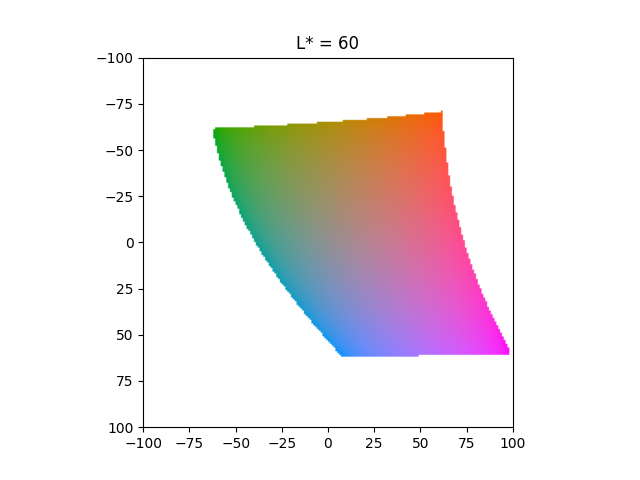
\includegraphics[width=\linewidth]{plot/lab_bins/60}
	\end{subfigure}
	\begin{subfigure}{.24\textwidth}
		\centering
		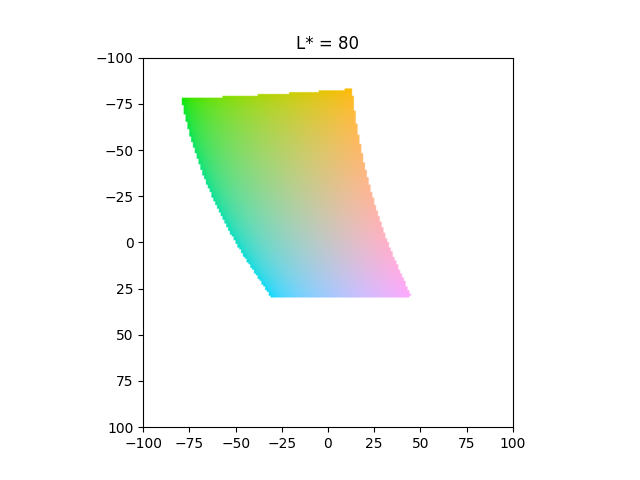
\includegraphics[width=\linewidth]{plot/lab_bins/80}
	\end{subfigure}
    \caption{Quantized \textbf{a*b*} bins for different \textbf{L*} values}
	\label{fig:lab_bins}
\end{figure}

Instead of predicting the exact \textbf{a*} and \textbf{b*} channel values 
for each pixel, this model outputs a probability distribution over 313 seperate classes. 
Each class represents one quantized \textbf{a*b*} bin. 
The $Q$-bins, each $10\times10$ in size, cover the whole \textbf{a*b*} gamut as seen
in figure \ref{fig:lab_bins}.

\begin{figure}[!ht]
	\centering
	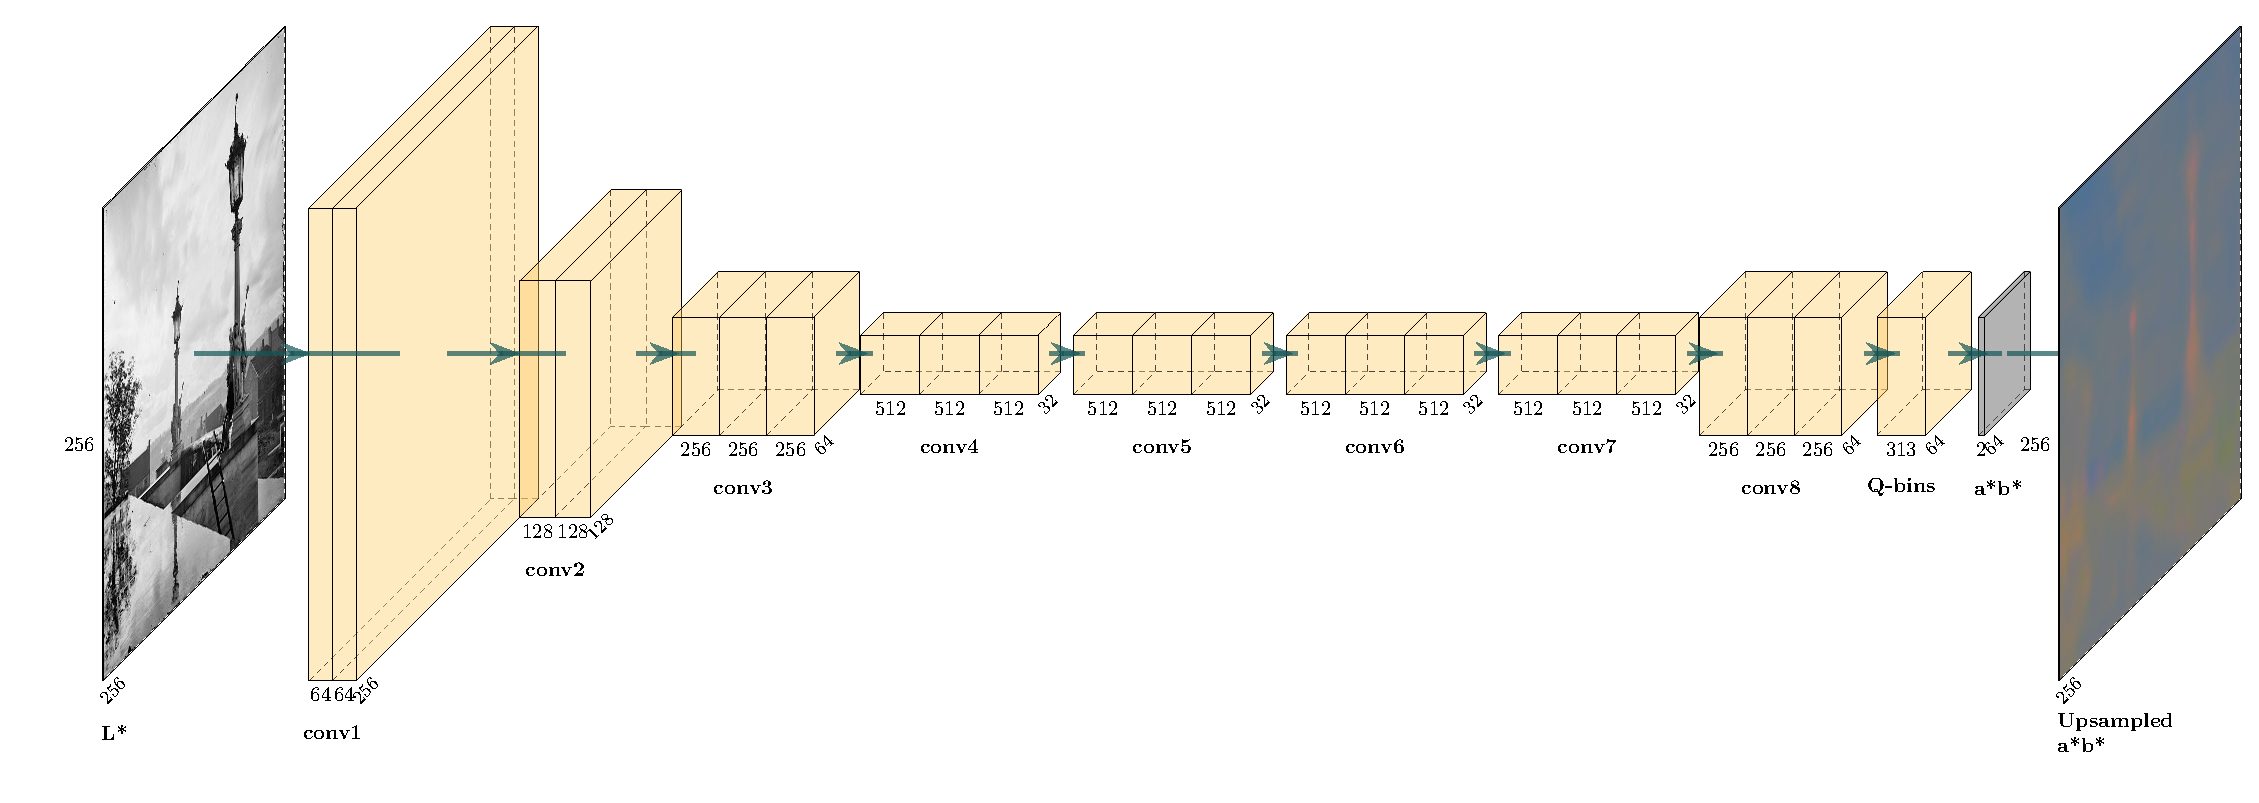
\includegraphics[width=\linewidth]{architecture/colorful}
    \caption{The architecture of the \textit{Colorful Image Colorization} model. 
	The eight convolutional blocks and the layer mapping the output to the probability 
	distribution over the $Q$-bins are colored in yellow, and probability to \textbf{a*b*}
	mapping in black}
	\label{fig:architecture_colorful}
\end{figure}

The model used is a modified version of the VGG \citep{simonyan2015vgg} network 
that was specifically created for classification. The model consists of eight
convolutional blocks and a convolutional-softmax pair for mapping the output to a
probability distribution over the 313 $Q$-bins.	All the convolutional blocks
consist of two to three convolutional-ReLU pairs (convolutional layer
paired with a ReLU activation \citep{abien2018relu}) and a batch normalization layer 
\citep{ioffe2015batchnorm} for normalizing the output of the block. 
The convolutional layers are all padded and have a kernel of size $3\times3$. There are 
no pooling layers in the network, the downsampling in the first three convolutional blocks 
is done by setting the stride in the last convolutional layer to $2$ instead.
To further increase the receptive field of each output distribution, à trous convolution
\citep{yu2016atrous} is used in the fifth and sixth layer, with the dilation set to $2$. 
Looking at the architecture of the network in figure \ref{fig:architecture_colorful},
we can see that the features are getting upsampled in the eighth block. The upsampling
is done by replacing the first layer of the block with a transposed convolution layer.
After the eighth block, a final convolution paired with softmax is applied to the 
features to get the probability distribution over the $Q$-bins. 

\subsection{Annealed mean}

To obtain the value of the \textbf{a*} and \textbf{b*} channels we could 
simply select the most likely color suggested by the colorizer On 
the other hand, we could calculate the weighted average over all the classes.
Somewhere in the middle of the two approaches lies the method proposed by 
the authors, they suggest a softmax-like calculation they named the annealed mean.
Using the annealed mean allows us to regulate how much we want to emphasize the 
most likely colors, or how close we want the result to be to the weighted 
average of the distribution.

Using the formula:

\begin{equation}
    W_T(p) = \frac{exp(log(p)/T)}{\sum_{q}{exp(log(p_q)/T)}}\label{eq:annealed_mean}
\end{equation}

we calculate the adjusted weights, where $p$ is the associated 
probability of a bin being the proposed color. $T$, which stands 
for temperature, is a hyperparameter of the function and it is used to 
adjust how drastically we want the colorization to be. When $T$ is set $1$
the weight is not adjusted and is equal to the probability $p$. On
the other hand, $T=0$ is an edge case where only the most probable bin 
gets assigned the weight of $1$. Programmatically that represents a problem 
as division  by zero results in an error, hence we implement a special case
for that situation where we map the probability distribution $\mathbf{p}$
to a one-hot encoded vector, with $1$ assigned to the $argmax(\mathbf{p})$
class.

As the sum over all the adjusted weights is $1$, the final color $\mathbf{c}$ 
for the pixel, given the probability distribution $\mathbf{p}$ is calculated 
using the formula:

\begin{equation}
    \mathbf{c} = \sum_{q}W_T(p_q) * \mathbf{c_q}\label{eq:weighed sum}
\end{equation}

\begin{figure}[!ht]
	\centering
	\begin{subfigure}{.19\textwidth}
		\centering
		\includegraphics[width=\linewidth]{img/colorful/temperature/100}
		\caption{$T=100$}
	\end{subfigure}
	\begin{subfigure}{.19\textwidth}
		\centering
		\includegraphics[width=\linewidth]{img/colorful/temperature/70}
		\caption{$T=70$}
	\end{subfigure}
	\begin{subfigure}{.19\textwidth}
		\centering
		\includegraphics[width=\linewidth]{img/colorful/temperature/40}
		\caption{$T=40$}
	\end{subfigure}
	\begin{subfigure}{.19\textwidth}
		\centering
		\includegraphics[width=\linewidth]{img/colorful/temperature/20}
		\caption{$T=20$}
	\end{subfigure}
	\begin{subfigure}{.19\textwidth}
		\centering
		\includegraphics[width=\linewidth]{img/colorful/temperature/0}
		\caption{$T=0$}
	\end{subfigure}
	\caption{Colorization of an image using different values of $T$}
	\label{fig:temperature}
\end{figure}

The effect that different values of $T$ have on the result of the colorization
can be seen in figure \ref{fig:temperature}. In the paper, the authors mention
that they got the best results using $T=0.38$. While that value might be the best
in general for fully automated colorization, individual photographs might benefit
from fine-tuning the hyperparameter. Higher temperature values usually result in 
lower overall saturation, while lower values yield crispier, but also more error-prone, results.

\begin{figure}[!ht]
	\centering
	\begin{subfigure}{.49\textwidth}
		\centering
		\includegraphics[width=\linewidth]{img/lab_channels/nature}
	\end{subfigure}
	\begin{subfigure}{.49\textwidth}
		\centering
		\includegraphics[width=\linewidth]{img/lab_channels/nature_4}
	\end{subfigure}
    \caption{Original image on the left, and the same image where the resolution of the \textbf{a*} and \textbf{b*} channels was reduced by a factor of four on the right}
	\label{fig:color4}
\end{figure}

In the end, the size of the output is 4 times smaller than the size of the input. 
Because of that, we upscale the output by a factor of 4 in the final step. That might
seem like a problem at first, but looking at figure \ref{fig:color4} we can see
that the \textbf{L*} channel is responsible for conveying most of the information, and
that the lower resolution of the \textbf{a*} and \textbf{b*} channels does not impact
the quality too much.

\subsection{Training}
\label{sec:colorful_training}

The network was trained on the ImageNet dataset that, when filtered, contains
1.1 million photographs of different shapes and sizes. Before training, we first
have to do a little preprocessing to make the process of training easier. It is 
preferable that all the inputs are of the same size, as training batches on 
different-sized images cannot be done efficiently, hence all the images were 
converted to a uniform size. 

\begin{figure}[!ht]
	\centering
	\includegraphics[width=0.8\linewidth]{img/colorful/resize}
    \caption{
	The image is first resized to a size where the shorter of the two sides
	is $256$ pixels in length, afterwards a $256\times256$ square is 
	randomly cropped out of the resized image}
	\label{fig:crop}
\end{figure}

The only is the restriction for the input size is that both the width and height
of the input image should be a multiple $8$ for the model to work. That restriction
is present because of the downsampling in the first three convolutional blocks of
the network. When selecting the input size, we need to take into account that the
model has to have a good enough resolution to detect which objects are present. On 
the other hand, the resolution of the images should not be too high as that slows 
down the training process. The size of $256\times256$ is a good compromise between
the two conditions, as the network will have more than enough information to colorize, 
but also the process of training will not take an eternity. The process of resizing 
can be seen in figure \ref{fig:crop}.

The model was trained for 600 thousand iterations using the Adam optimizer \citep{diederik2015adam}
with a batch size of 40. The initial learning rate was $3\times10^-4$, and it was
reduced by a factor of $\sim$3 ($3\times10^{-4}$, $1\times10^{-4}$, $3\times10^{-5}$,
..., $1\times10^{-6}$) every 100 thousand iterations, or roughly every 4 epochs. 
Throughout the training, the optimizer parameters were static with the weight decay
being set to $1\times10^{-3}$ and $\beta_1$, $\beta_2$ having the value of $(0.9, 0.99)$.

\begin{algorithm}[!ht]
	\caption{Training step for the \textit{Colorful Image Colorization} model}
	\label{alg:colorful}
	\begin{algorithmic}		
		\Function {step}{$batch$, $network$, $optimizer$}		
			\State $l \leftarrow batch[:1]$	
			\State $ab \leftarrow batch[1:]$
			\State $predicted \leftarrow network.forward(l)$	
			\State $q\_bins \leftarrow encode(ab)$
			\State $loss \leftarrow CELoss(predicted, q\_bins)$
			\State $loss.backward()$
			\State $optimizer.step()$
		\EndFunction
	\end{algorithmic}
\end{algorithm}

One training step of the colorizer is outlined in figure \ref{alg:colorful}. 
Firstly we separate the \textbf{L*} from the \textbf{a*b*} channels, as \textbf{L*}
is the input, and \textbf{a*} and \textbf{b*} are wanted outputs. Next, 
we carry out a forward pass through the network and get the proposed color 
distribution for the images. At this point, we cannot calculate the loss of the
colorization as the \textbf{a*} and \textbf{b*} have to be encoded into 313 bins.
After the encoding we calculate the cross-entropy, calculate the gradients, and 
update the model.

\begin{figure}[!ht]
	\centering
	\includegraphics[width=0.5\linewidth]{img/colorful/distribution}
    \caption{Graph borrowed from the original paper \citep{zhang2016colorful}, 
	showing the overall distribution of color channel values in the ImageNet
	dataset, using a logarithmic scale (red indicates high, and blue low occurance)}
	\label{fig:distribution}
\end{figure}

The encoding of \textbf{a*} and \textbf{b*} could be done by finding the 
closest $Q$-bin and creating a one-hot vector representing that color. The 
problem with that representation is that we cannot express if the color
was somewhere in between of two bins. That's why the authors of the 
paper proposed encoding the color by applying a Gaussian kernel. That way
the closer the color is to the center of the bin the higher the associated
value of the class is. Another useful property of this encoding is that this way
the network can learn which bins are neighboring, as the encoder will only 
activate neighboring classes at the same time.

Unfortunately, the cross-entropy loss is usually implemented using labels as targets,
and not encoded vectors. While that approach is quite optimized and much faster, 
it does not suit our needs as we are soft-encoding the colors. That's why for 
the purpose of training this model we have to implement a custom multinomial 
cross-entropy loss.

Looking at figure \ref{fig:distribution} we can see that the colors are not 
equally distributed over the \textbf{L*a*b*} color space, on the contrary
the neutral colors (the ones closer to the center of the graph) are represented
at a much higher rate than marginal colors. To counter that disparity we can
rebalance the classes \citep{tantithamthavorn2020rebalancing}, giving the 
underrepresented classes an equal chance to get selected.

\subsection{Results}

\clearpage
\section{Generative Adversarial Networks for Colorization}
\label{sec:gan}

The second approach to colorization analyzed in this thesis comes in the form
of a generative adversarial network (abbr. \textit{GAN}) \citep{goodfellow2014generative}.
The main motivation for using GANs in this scenario is beacause of the 
generator-discriminator schema which has proven its usefulness in generating 
convincing data. The paper by Nazeri et al. was used as the main reference, 
but the paper by Isola et al. strongly influenced some training choices.

\subsection{Architecture}

The architecture of this model was ispired by the \textit{pix2pix} model proposed
by Isola et al. in 2017 for image-to-image translation tasks. Image colorization
was mentioned as one of many potential use cases for their model.

\subsubsection{Generative adversarial networks}

Generative adversarial networks are based on the idea of a \textit{game} between
two artificial neural networks. The first of the two networks, called the generator, 
has the task of generating plausible-looking data. The second network, called the
discriminator, has to discern if the data it got was artificially generated by the
generator, or if it is genuine data.

\begin{figure}[!ht]
	\centering
	\includegraphics[width=0.7\linewidth]{img/gan/museum}
    \caption{Analogy for the way GANs work}
	\label{fig:museum}
\end{figure}

The tasks of the two networks can be thought of as a rivalry between a forger
and a museum examiner outlined in figure \ref{fig:museum}. The goal of the forger
is to create forgery that cannot be identified as being a forgery, and the goal 
of the examiner is to discern artworks from forgeries.

It all starts with the forger that submits an artwork, that does not make any 
sense, to the museum. The artwork finds its way to the examiner who decides 
it is a forgery, and he explains to the forger the mistakes he made.
The forger, armed with new information on how his forgery attempt was detected, 
heads out and creates a new forgery that, hopefully, addresses the flaws of the
last one. Again he submits the forgery to the museum where the cycle continues
until the forger manages to produce convincing forgeries.

The main problem in that analogy is that we usually do not have a perfect 
discriminator that can discern a forgery from an artwork. That is why 
we train the generator and discriminator at the same time from scratch. The 
discriminator, which is a binary classifier, is trained on examples of real 
and fake (created by the generator) data and has to decide what belongs 
to which class. On the other hand, the usual way to train a generator is a bit
more complicated. First, a forward pass is done through the generator, and then 
the generated data is forwarded through the discriminator. Because we want our 
generator to be nudged in the direction so it generates convincing fake data, we
calculate the loss with the label set as if it was real data. Next, the gradients are
pulled through the discriminator and the generator. In the last step, we update
only the generator weights.

\begin{figure}[!ht]
	\centering
	\begin{subfigure}{.49\textwidth}
		\centering
		\includegraphics[width=\linewidth]{img/gan/mnist}
	\end{subfigure}
	\begin{subfigure}{.49\textwidth}
		\centering
		\includegraphics[width=\linewidth]{img/gan/mnist_collapsed}
	\end{subfigure}
    \caption{A successful result of a GAN trained on the MNIST dataset on the left, 
	and an unsuccessful attempt that ended up in mode collapse on the right}
	\label{fig:gan_mnist}
\end{figure}

A flaw in the GAN framework is the so-called mode collapse (or Helvetica scenario) 
demonstrated in figure \ref{fig:gan_mnist}. As the name suggests, mode collapse is 
a situation where the generator finds only one possible solution to the problem 
that satisfies the discriminator. At that moment, when the generator is specialized
in reproducing one answer, and the discriminator is not able to discern it from 
the original, the generator cannot learn anything new and just further specializes
in reproducing the existing answer.

\subsubsection{Conditional GAN}

\begin{figure}[!ht]
	\centering
	\includegraphics[width=0.5\linewidth]{img/gan/mnist_cgan}
    \caption{Generating fake hand-written digits based on the MNIST dataset 
	using the cGAN framework. Digits in the same row are generated using 
	the same latent vector (seed), and demonstrate similar characteristics}
	\label{fig:cgan_mnist}
\end{figure}

Conditional generative adversarial networks (abbr. \textit{cGAN})\citep{mirza2014cgan}
are an extension to the typical adversarial network paradigm proposed not long 
after the original GAN paper was published. In the cGAN network, both the generator
and the discriminator are conditioned with the same input data.
In the case of generating fake hand-written digits based on the MNIST \citep{lecun2010mnist}
dataset, proposed in the original GAN paper \citep{goodfellow2014generative}
one of the problems is that we could not force the generator to create images
of a certain class which sometimes ended up in mode collapse. That problem can be 
solved using cGANs by adding a conditional variable to the generator and 
discriminator. That way the generator had the information on what digit to create, 
while the discriminator knew which digit was supposed to be on the input. An 
example of the output of a trained cGAN model can be seen in the figure \ref{fig:cgan_mnist}.

In the case of colorization, the conditional variable is the grayscale input, 
that way the generator knows what it has to colorize, while the discriminator
knows what is supposed to be colorized.

\subsubsection{Generator}

\begin{figure}[!ht]
	\centering
	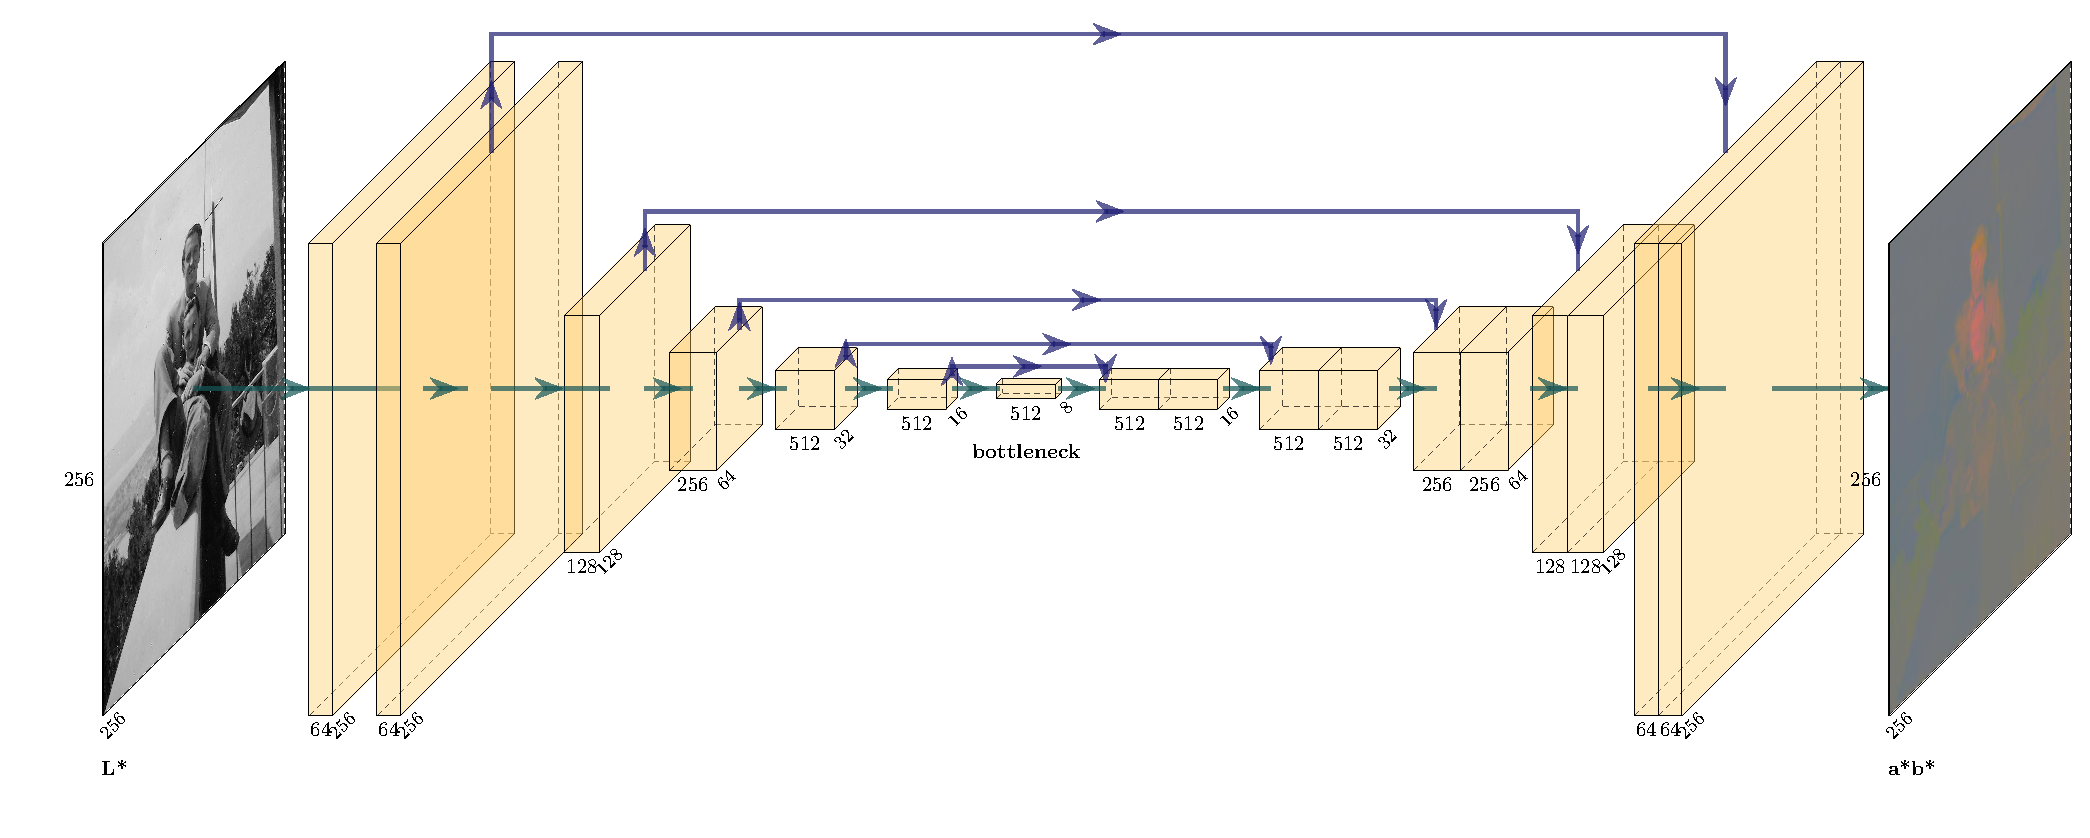
\includegraphics[width=\linewidth]{architecture/gan_generator}
    \caption{The U-Net architecture of the model used for the generator, the short connection
	is done by concatenating the features from the encoder to the de-convoluted features
	of the previous layer in the decoder.}
	\label{fig:architecture_gan}
\end{figure}

For the generator, a U-Net-style network was selected. The encoder consists
of 5 consecutive convolutional layers that halve the spatial dimensions. The 
number of feature channels is doubled in the first three convolutional layers, 
at which point it stays at 512 feature channels until the bottleneck. The decoder
is almost perfectly symmetrical, except for the fact that the input dimensions for 
the transposed convolutions are double the size. The reason for the doubled input
size is because the short connections are achieved by concatenating the features
from the encoder with the features from the last transposed convolution. The architecture
of the network is depicted in the diagram \ref{fig:architecture_gan}.

\subsubsection{Discriminator}

\begin{figure}[!ht]
	\centering
	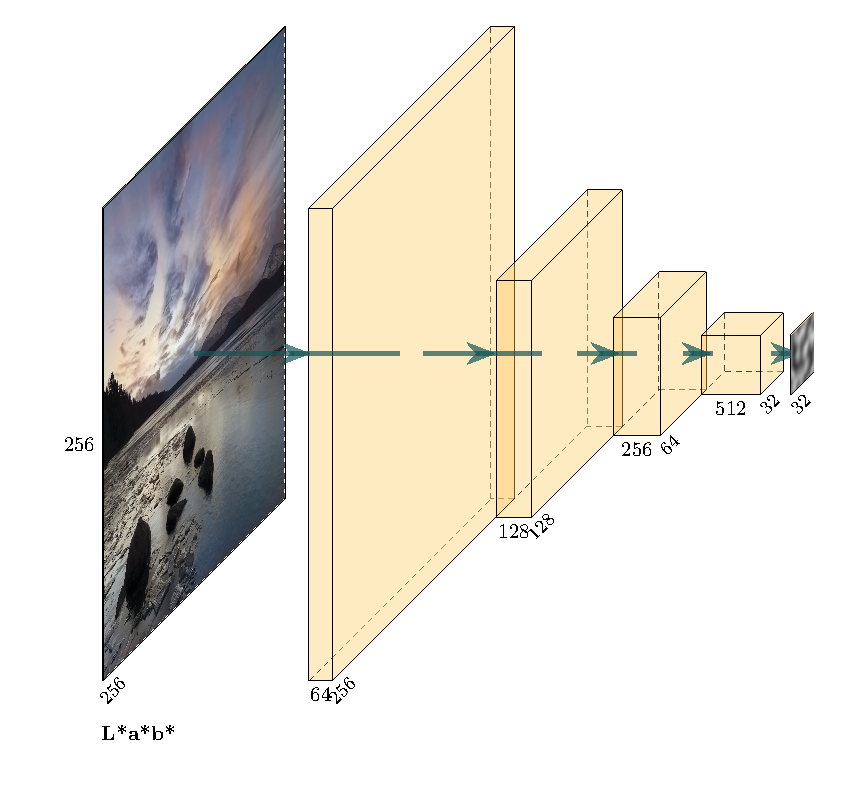
\includegraphics[width=0.5\linewidth]{architecture/gan_discriminator}
    \caption{The patch-GAN discriminator architecture}
	\label{fig:architecture_gan_discriminator}
\end{figure}

The discriminator network for this GAN is a simple fully convolutional neural network.
As it can be seen in figure \ref{fig:architecture_gan_discriminator}, the output
of the discriminator is not a single scalar, but a $32\times32$ array
where each value is the discriminators guess if a specific patch of the input is 
genuine or not. Because of the patchy approach to the classification of the input, 
GANs using this kind of discriminators are called PatchGANs \citep{isola2017pix2pix}.

\begin{figure}[!ht]
	\centering
	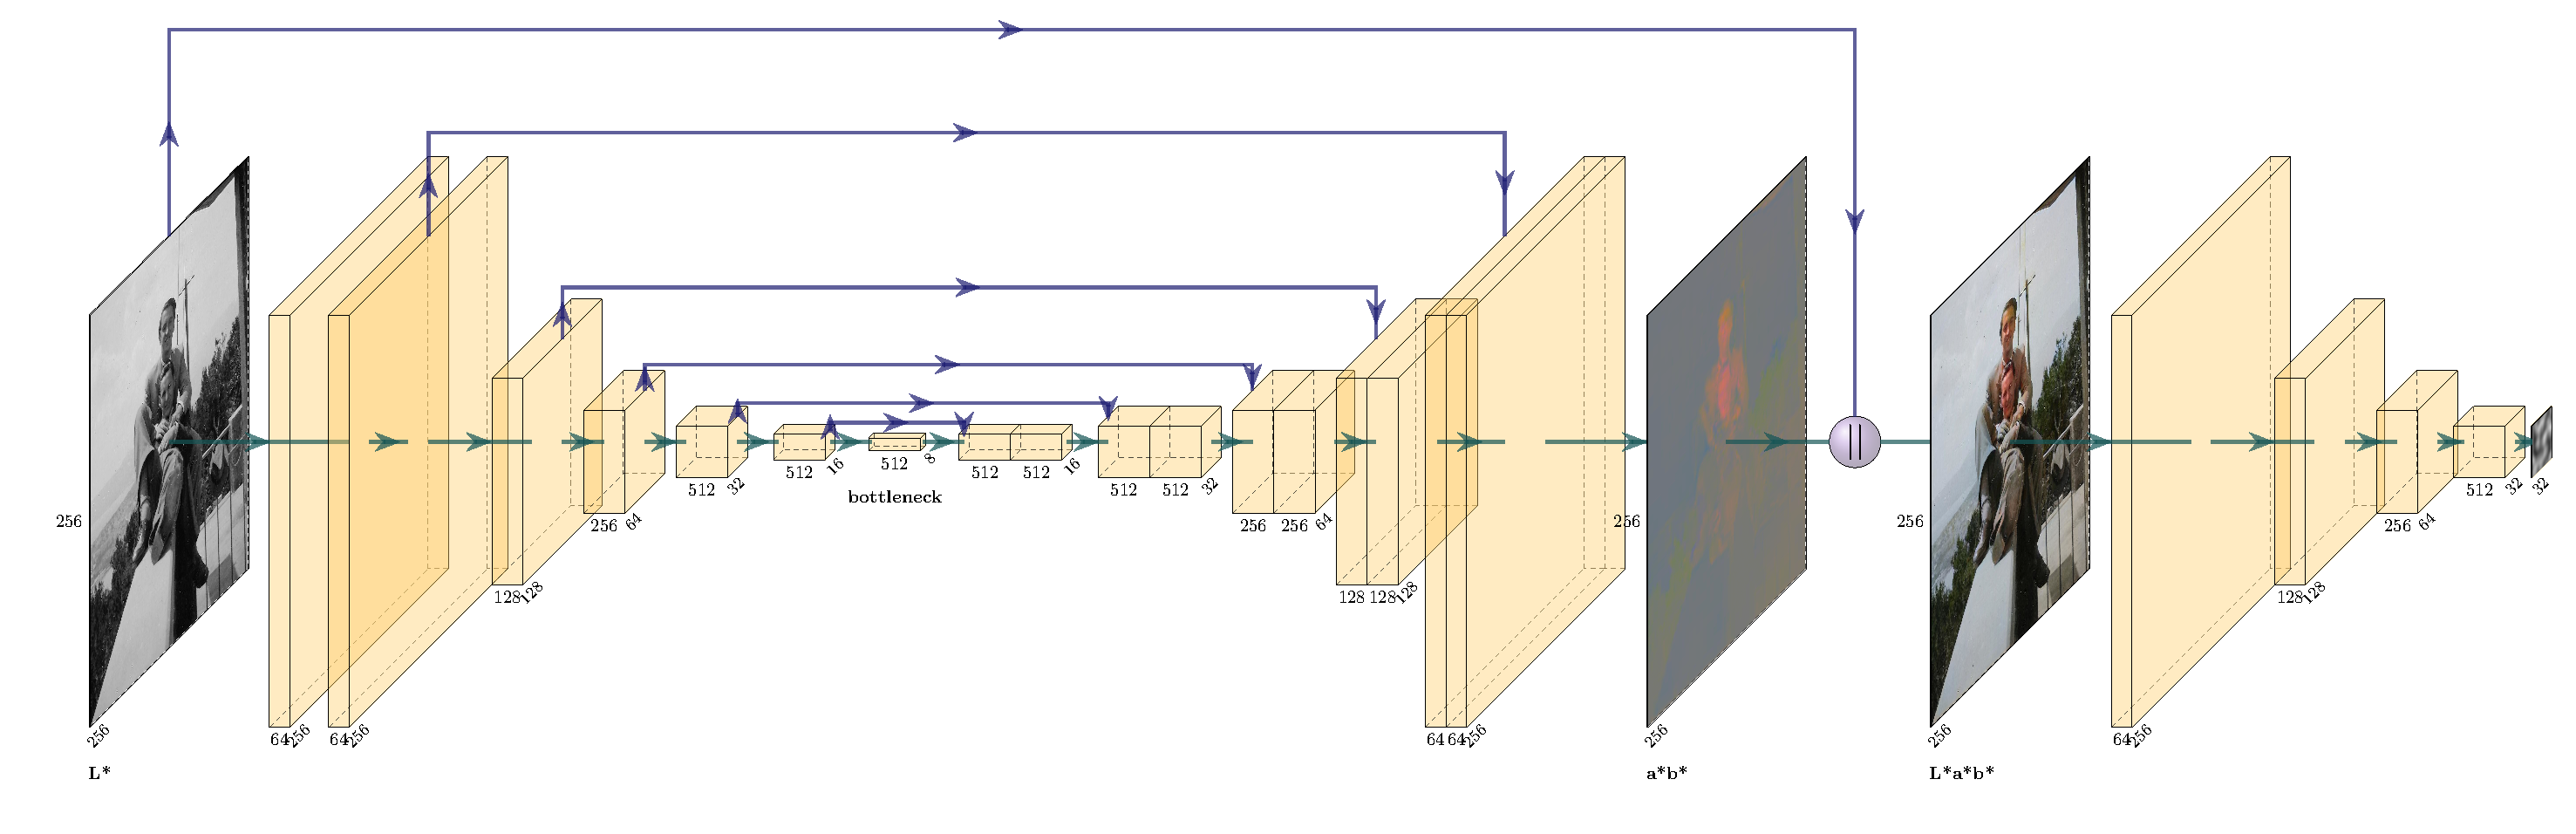
\includegraphics[width=\linewidth]{architecture/gan_full}
    \caption{The patch-GAN discriminator architecture}
	\label{fig:architecture_gan_full}
\end{figure}

With the generator and discriminator described, the diagram of the whole GAN can
be seen in \ref{fig:architecture_gan_full}


\subsection{Training}

Although the loss function for traing the generative adversarial networks can be neatly 
written down as a minimax game between the generator $G(\mathbf{l};\theta_G)$ and the 
discriminator $D(\mathbf{l, ab};\theta_D)$:
\begin{equation}
	\min_{G}\max_{D}V(D,G)=\mathbb{E}[L(D(\mathbf{l, ab}))] + \mathbb{E}[-L(D(\mathbf{l}, G(\mathbf{l}))) + \lambda \cdot \mathit{L_1}(G(\mathbf{l}), \mathbf{ab})]
\end{equation}
, the actual process of training is not that simple. In the addition to the gradients 
the generator gets via the discriminator, we calculate the $\mathit{L_1}$ loss between
the output of the generator and the expected value. The $\mathit{L_1}$ loss is then 
multiplied with the hyperparameter $\lambda$ to scale the gradients.

\begin{algorithm}[!ht]
	\caption{Training step for the \textit{Colorful Image Colorization} model}
	\label{alg:gan}
	\begin{algorithmic}		
		\Function {step}{$batch$, $G$, $D$, $opt_G$, $opt_D$}
			\State $l \leftarrow batch[:1]$	
			\State $ab \leftarrow batch[1:]$
			\State $predicted \leftarrow G(l)$
			\State $fake \leftarrow D(l, predicted)$
			\State $real \leftarrow D(l, ab)$
			\State $loss_D \leftarrow (BCELoss(fake, 1) + BCELoss(real, 0))/2$
			\State $loss_D.backward()$
			\State $opt_D.step()$
			\State $loss_G \leftarrow \lambda * L1Loss(predicted, ab) - BCELoss(fake, 0)$
			\State $loss_G.backward()$
			\State $opt_G.step()$
		\EndFunction
	\end{algorithmic}
\end{algorithm}

As with the \textit{Colorful Image Colorization} model, we have to do the same sort of 
preprocessing as described in section \ref{sec:colorful_training}, to bring the training
data to a uniform size. Afterward, one step of the training process goes as described in 
function \ref{alg:gan}. As suggested by the authors of the paper, several strategies 
were used to encourage the generator to produce better results.

The first strategy used is the modified loss function that was proposed by Ian Goodfellow
in the 2016 NIPS tutorial \citep{goodfellow2017nips}, where instead of minimizing 
the chance of the discriminator being correct, we maximize the chance of the discriminator 
being mistaken. Although that might sound like it is the same thing, the difference 
is in the steepness of the gradient that is forwarded to the generator. Namely, if the 
discriminator performs well early on, the generator will have near-zero gradients
during backpropagation. On the other hand, maximizing the chance of the discriminator
being mistaken results in a non-saturated game between the two networks.

In addition to the modified loss function, one-sided label smoothing was used 
\citep{salimans2016improved_gans}. With label smoothing, the label for the \textit{false} and 
\textit{true} value is not set to 0 and 1, but to a slightly higher/lower value (eg. 0.1, 0.9). 
One-sided smoothing is a half-way approach, where the \textit{false} label remains 0, but the 
true label is smoothed. Using label smoothing was shown to reduce the vulnerability of 
neural networks to adversarial examples.

\begin{figure}[!ht]
	\centering
	\includegraphics[width=\linewidth]{img/gan/gan_plot}
    \caption{Healthy back and forth between the generator and the discriminator. 
	Discriminator error on real samples in red, and on fake samples in blue.}
	\label{fig:gan_plot}
\end{figure}

Although it is hard to estimate if the training of the generator is going well, there 
are some indicators of good behavior. Usually, we could look at the $L1$ error of 
the predicted \textbf{a*} and \textbf{b*} channels, but due to multimodality, that 
value stagnates at a very early stage of training. On the other hand, looking at 
figure \ref{fig:gan_plot} we can see what a healthy \textit{relationship} between
the generator and the discriminator should look like. The losses of the real and fake 
samples fluctuate up and down as a result of the game between the generator and 
the discriminator, but they generally stay at the same level.

\subsection{Results}

\clearpage
\section{Interactive Deep Colorization}
\label{sec:ideep}

The last of the three models analyzed is the \textit{Interactive Deep Colorization}
model proposed by Zhang et al. in 2017, and it builds on the model described 
in section \ref{sec:colorful}. It differs from the \textit{Colorful Image Colorization}
and the GAN-based model in that it is semi-automated. It can work as a fully-automated model, 
but in general much better results are acheived when the model is operated by a human. 

In the paper two models were proposed, out of which only one was analyzed for this thesis. 
The selected model gets additional information about the desired colorization in the 
shape of so-called global hints described in section \ref{sec:global}.

\subsection{Architecture}

\begin{figure}[!ht]
	\centering
	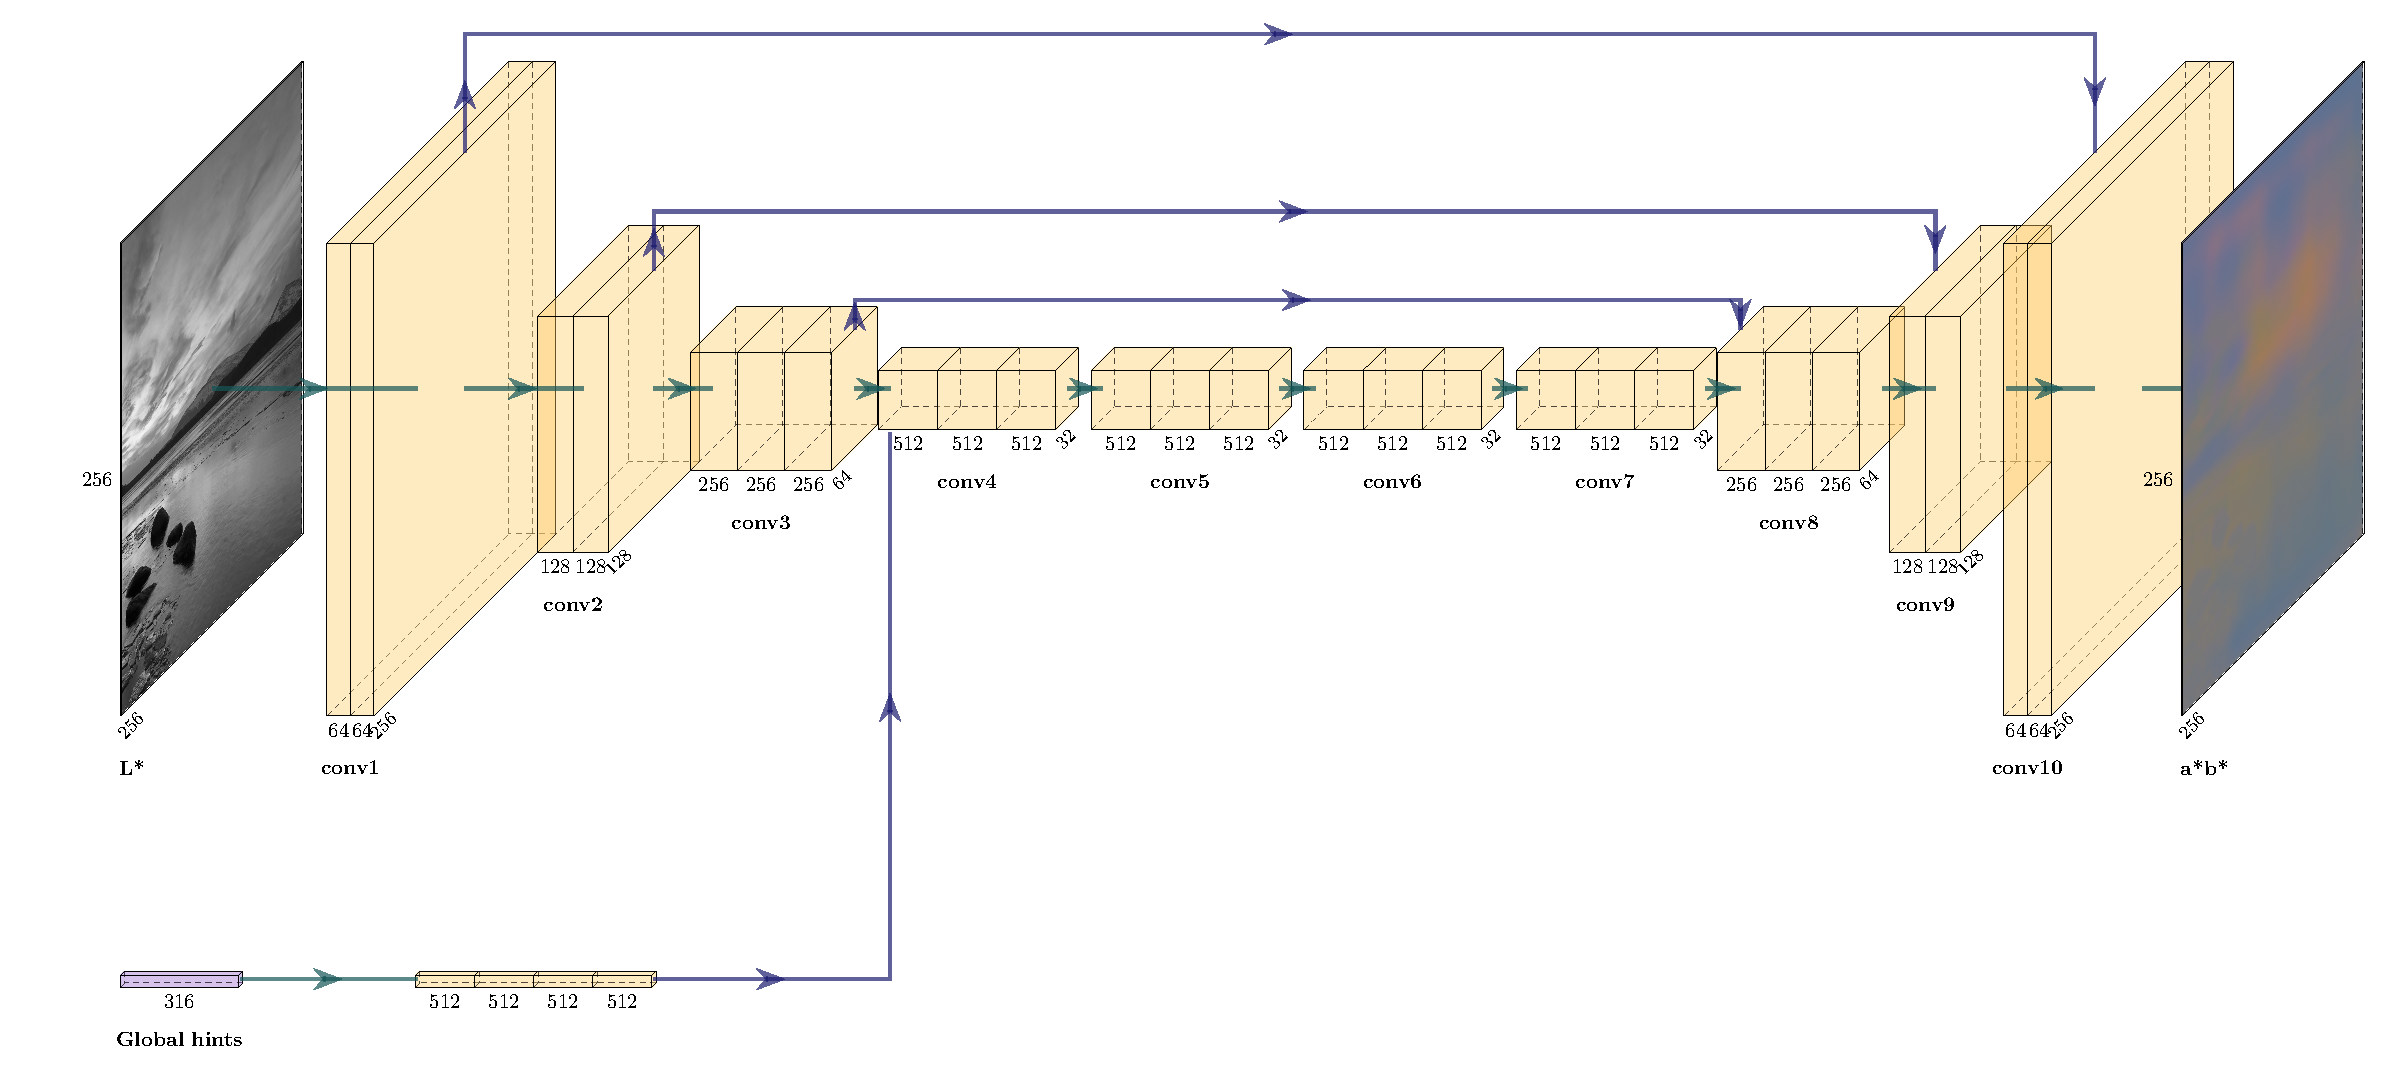
\includegraphics[width=\linewidth]{architecture/ideep}
    \caption{The architecture of the \textit{Interactive Deep Colorization} network. 
	The base \textit{Colorful Image Colorization} network is highlighted in red, the new 
	layers are yellow, and the global hints network is colored purple.}
	\label{fig:architecture_ideep}
\end{figure}

The architecture of the first model can be seen in the figure \ref{fig:architecture_ideep}, 
and it is an extended version of the model described in section \ref{sec:colorful_architecture}. 
In the figure, the \textit{Colorful Image Colorization} model is colored in red, while 
the new elements are colored yellow/purple. The yellow blocks are the new convolutional 
blocks, while the purple block is the global hints network that will be further described
in section \ref{sec:global}.

The model was extended with two convolutional blocks that further upscale the resolution 
of the output. The problem of the bottleneck, which arose from the information loss in the 
first three layers, was solved by adding three skip connections between first and last three
blocks. By adding the skip connections, we essentially converted the VGG-style model to a
U-Net.


Although it is not visible in the diagram, the skip connections were not realized by 
simply concatenating the output features of the first layers to the inputs of the 
last layer, but instead the feture transfer was done by addition. But, before adding 
up the shorted connections, they were first forwarded through a convolutional layer.



\clearpage
- additional 2 expansive layers + skip connections and skip convolutions + global hints

\subsection{Transfer learning}

- What is transfer learning:
	Dogradivanje
	- Training one model and applying the learned knowledge on another model
	
- The weights of the trained first model, in the end crucial as the model could not colorize without the initial push

\subsection{Global hints}
\label{sec:global}


\subsection{Training}

\subsection{Results}